\section{Background}
\label{sec:background}
This section gives a brief overview of the theoretical considerations and concepts related to Monte-Carlo Tree Search. These ideas will be extended in Section \ref{sec:variations} and Section \ref{sec:use_cases}.
\subsection{Game Theory}
\label{ss:game_theory}
Following the conventions used by Browne et al.\cite{browne2012survey} a game is formally modeled using the following components:
\begin{itemize}[noitemsep]
    \item $n \in \mathbb{N}$ players $k_1, \ldots, k_n$
    \item A set of states $S$ with an initial state $s_0$ and terminal states $S_T \subseteq S$
    \item A set of possible actions $A$
    \item A state transition function $f: S \times A \to S$
    \item A reward function $r: S \to \mathbb{R}^k$
\end{itemize}
A game starts in state $s_0$ and progresses according to the state transition function $f$ which at point $t$ gives us the next state $s_{t+1}$. Transitions happen through the action $a$ taken by a player $k_i$. Usually it is only one players' turn at any given point $t$. The reward function $r$ determines points gained or lost by players through these actions. The game ends when a terminal state $s_j \in S_T$ is reached. The probability of a given player choosing any action $a$ is determined by its \textit{policy} and may be constrained by the current state $s$ via the rules of the game. Games can be classified using the following criteria:
\begin{enumerate}[label=\alph*)]
    \item \textit{zero sum}: Do the rewards given to all players add up to zero?
    \item \textit{information}: Is the complete state of the game known to the players?
    \item \textit{determinism}: Does change play a part?
    \item \textit{sequential}: Can multiple players choose an action simultaneously?
    \item \textit{discreteness}: Are actions atomic or do they take time? 
\end{enumerate}
An important category of games are so-called \textit{combinatorial games}. They are zero-sum, perfect information, deterministic, sequential and discrete. Examples are \textit{Go}, \textit{Chess} and \textit{Tic-Tac-Toe}.

\subsection{Monte Carlo Methods and Multi Armed Bandits}
The basic idea of Monte-Carlo based methods is that of \textit{sampling}. While operating on a very large domain it is not feasible to simply do calculations which consider all possible elements of said domain. We therefore have to select only a (usually much smaller) subset of these elements to represent the domain somewhat accurately and to gain as much information as possible. In the context of games the aim of such methods is to find good moves while only analyzing some parts (states, actions and rewards) of the game. This can be done by starting at an initial state (either the actual first state or just the current game state) and repeatedly estimating the value of possible actions. The idea is that these estimations will converge and allow us to make an informed choice, that is, to choose a good action at a rate much higher than chance. One widely used concept when applying Monte Carlo methods to games is the so-called Q-value. At an action $a$ at a state $s$ it is defined as the expected reward of this action:
\begin{equation*}
    Q(s,a)= \frac{1}{N(s,a)} \sum_{i=1}^{N(s)} \mathbb{I}_i(s,a) \cdot Q^i(s)
\end{equation*}
$Q^i(s)$ is the result of the $i$-th simulation started from $s$, $N(s)$ denotes how often $s$ has been visited, $N(s,a)$ denotes how often action $a$ has been selected when $s$ has been visited and $\mathbb{I}_i(s,a)$ is one if $a$ has been selected when in state $s$ during the $i$-th simulation from $s$ and zero otherwise. Simulation in this context refers to a play-out of the game from the selected state, a more precise definition is given in later sections.


In a \textit{Multi-Armed-Bandit} problem (see e.g. \cite{lattimore2018bandit} for an introduction) a player has to choose one of $K$ actions (\enquote{arms}) out of the set $\mathcal{K} = \{1,\ldots,K \}$ at each one of $T$ rounds. The number of rounds $T$ is called the \textit{horizon} of the game and the decision points $t_1,\ldots,t_T$ are called the decision epochs. Each arm has a value associated with it. These rewards $X^k_t$ of arm $k$ at decision epoch $t$ can be modeled as a random variable with values $X_k^t \in [0,1]$ and expected value $\mu_t^k = \mathbb{E}[X^k_t]$. The best possible reward is therefore given via 
\begin{equation*}
\mu^\star_t = \max_{k \in \mathcal{K}} \{ \mu^k_t\}    
\end{equation*}
In the \textit{non-stationary} problem formulation the value of each arm may change over the course of the game. The extent of this change is called \textit{temporal variation}. The performance of a given policy (arm selection) can be measured relative to an oracle which has perfect information and picks the best possible choice. The difference in rewards between the policy and the oracle is called \textit{regret}. After n epochs it is given as:
\begin{equation*}
    R_n = \mu^\star n - \sum_{j=1}^K \mu^j \cdot \mathbb{E}[T_j(n)]
\end{equation*} $\mu^\star$ is the maximum reward mean, $\mu^j$ is the reward mean of arm $j$ and $\mathbb{E}[T_j(n)]$ is the expected number of times arm $j$ has been played in the first $n$ epochs. The regret can be seen as the difference between the performance of an oracle with complete information and an algorithm with incomplete information. Any policy aims to minimize this value. As shown by Lai and Robbins \cite{lai1985asymptotically} there exist no policy with a growth of the regret slower than $O(\ln n)$ for most reward distributions (i.e., distributions of the rewards $X^k_t$). For bandit problems it is desirable to know the \textit{Upper Confidence Bound} (UCB) that any given arm will be optimal in the game-theoretic sense described in Section \ref{ss:game_theory}. In the formulation of Sironi and Winands \cite{sironi2019comparing} (called UCB1) it is given by:
\begin{equation*}
    \text{UCB1} = \underbrace{Q(s,a)}_{(\ast)} +  \underbrace{\sqrt{\frac{2 \ln N(s)}{N(s,a)}}}_{(\ast \ast)}
\end{equation*}
Since this term is maximized by any reasonable policy (i.e., one that aims to win) its parts can be analyzed quite easily: The first term $(\ast)$ facilitates the exploration of higher reward choices while the second term $(\ast \ast)$ does the same for less-visited, currently deemed less promising choices. This term is prominently used as a sampling strategy in the UCT-MCTS variant described below. 
\subsection{Monte Carlo Tree Search}

All paths through a game, in the above definition, can be exhaustively described in the so-called \textit{game tree}. This (conceptual, theoretical) data structure is a tree that contains all possible states a game could be in. Its nodes represent the states and its edges $(s_i,s_j)$ represent the action leading from state $s_i$ to state $s_j$. In practice however, this tree is too large to actually be represented. For example, in chess there are about $35^{80}$ possible playthroughs and consequently as many paths through the game tree. Monte Carlo Tree Search (Algorithm \ref{alg:mcts_basic}) is an algorithm for traversing game trees utilizing the idea of sampling. MCTS iteratively builds a partial game tree (the \textit{search tree}) while a certain condition holds, usually referred to as the computational budget. In each iteration this current \enquote{view} of the game tree is refined by estimating and refining the value of the states contained. Consecutive iterations of MCTS usually represents a turn of a game-playing agent. That means the search is used to find the most valuable state. When the budget is exhausted and no more iterations are possible the action leading to this state (or, generally to a subtree containing it) is returned and executed by the agent. This will be the setting for the remainder of this paper but since MCTS is a general-purpose search algorithm for any problem that can be modeled as a game it may not be the specific purpose of every use case. This will become evident in Section \ref{sec:use_cases}. The algorithm consists of four basic steps displayed in Figure \ref{fig:mcts_basics}:
\begin{enumerate}[label=\arabic*)]
    \item \textit{Selection}: Beginning from the root node $t_0$ the tree is traversed using a child selection policy until an expandable node $t_n$ (representing state $s$) is reached: that is, a node representing a non-terminal state that has unvisited children.
    \item \textit{Expansion}: One or more child nodes are added to the tree if the actions leading to them are possible. Here, $t_l$ representing state $s'$ is added by selecting action $a$. 
    \item \textit{Simulation}: From the state of the new node a simulation of the game is run according to the \textit{Default Policy}. Its results are taken to be the value of the node.
    \item \textit{Backpropagation}: The new values are backed up through the tree which may result in updates to the statistics of the nodes. This means updating the Q-values.
\end{enumerate}
\begin{figure}[ht]
    \centering
    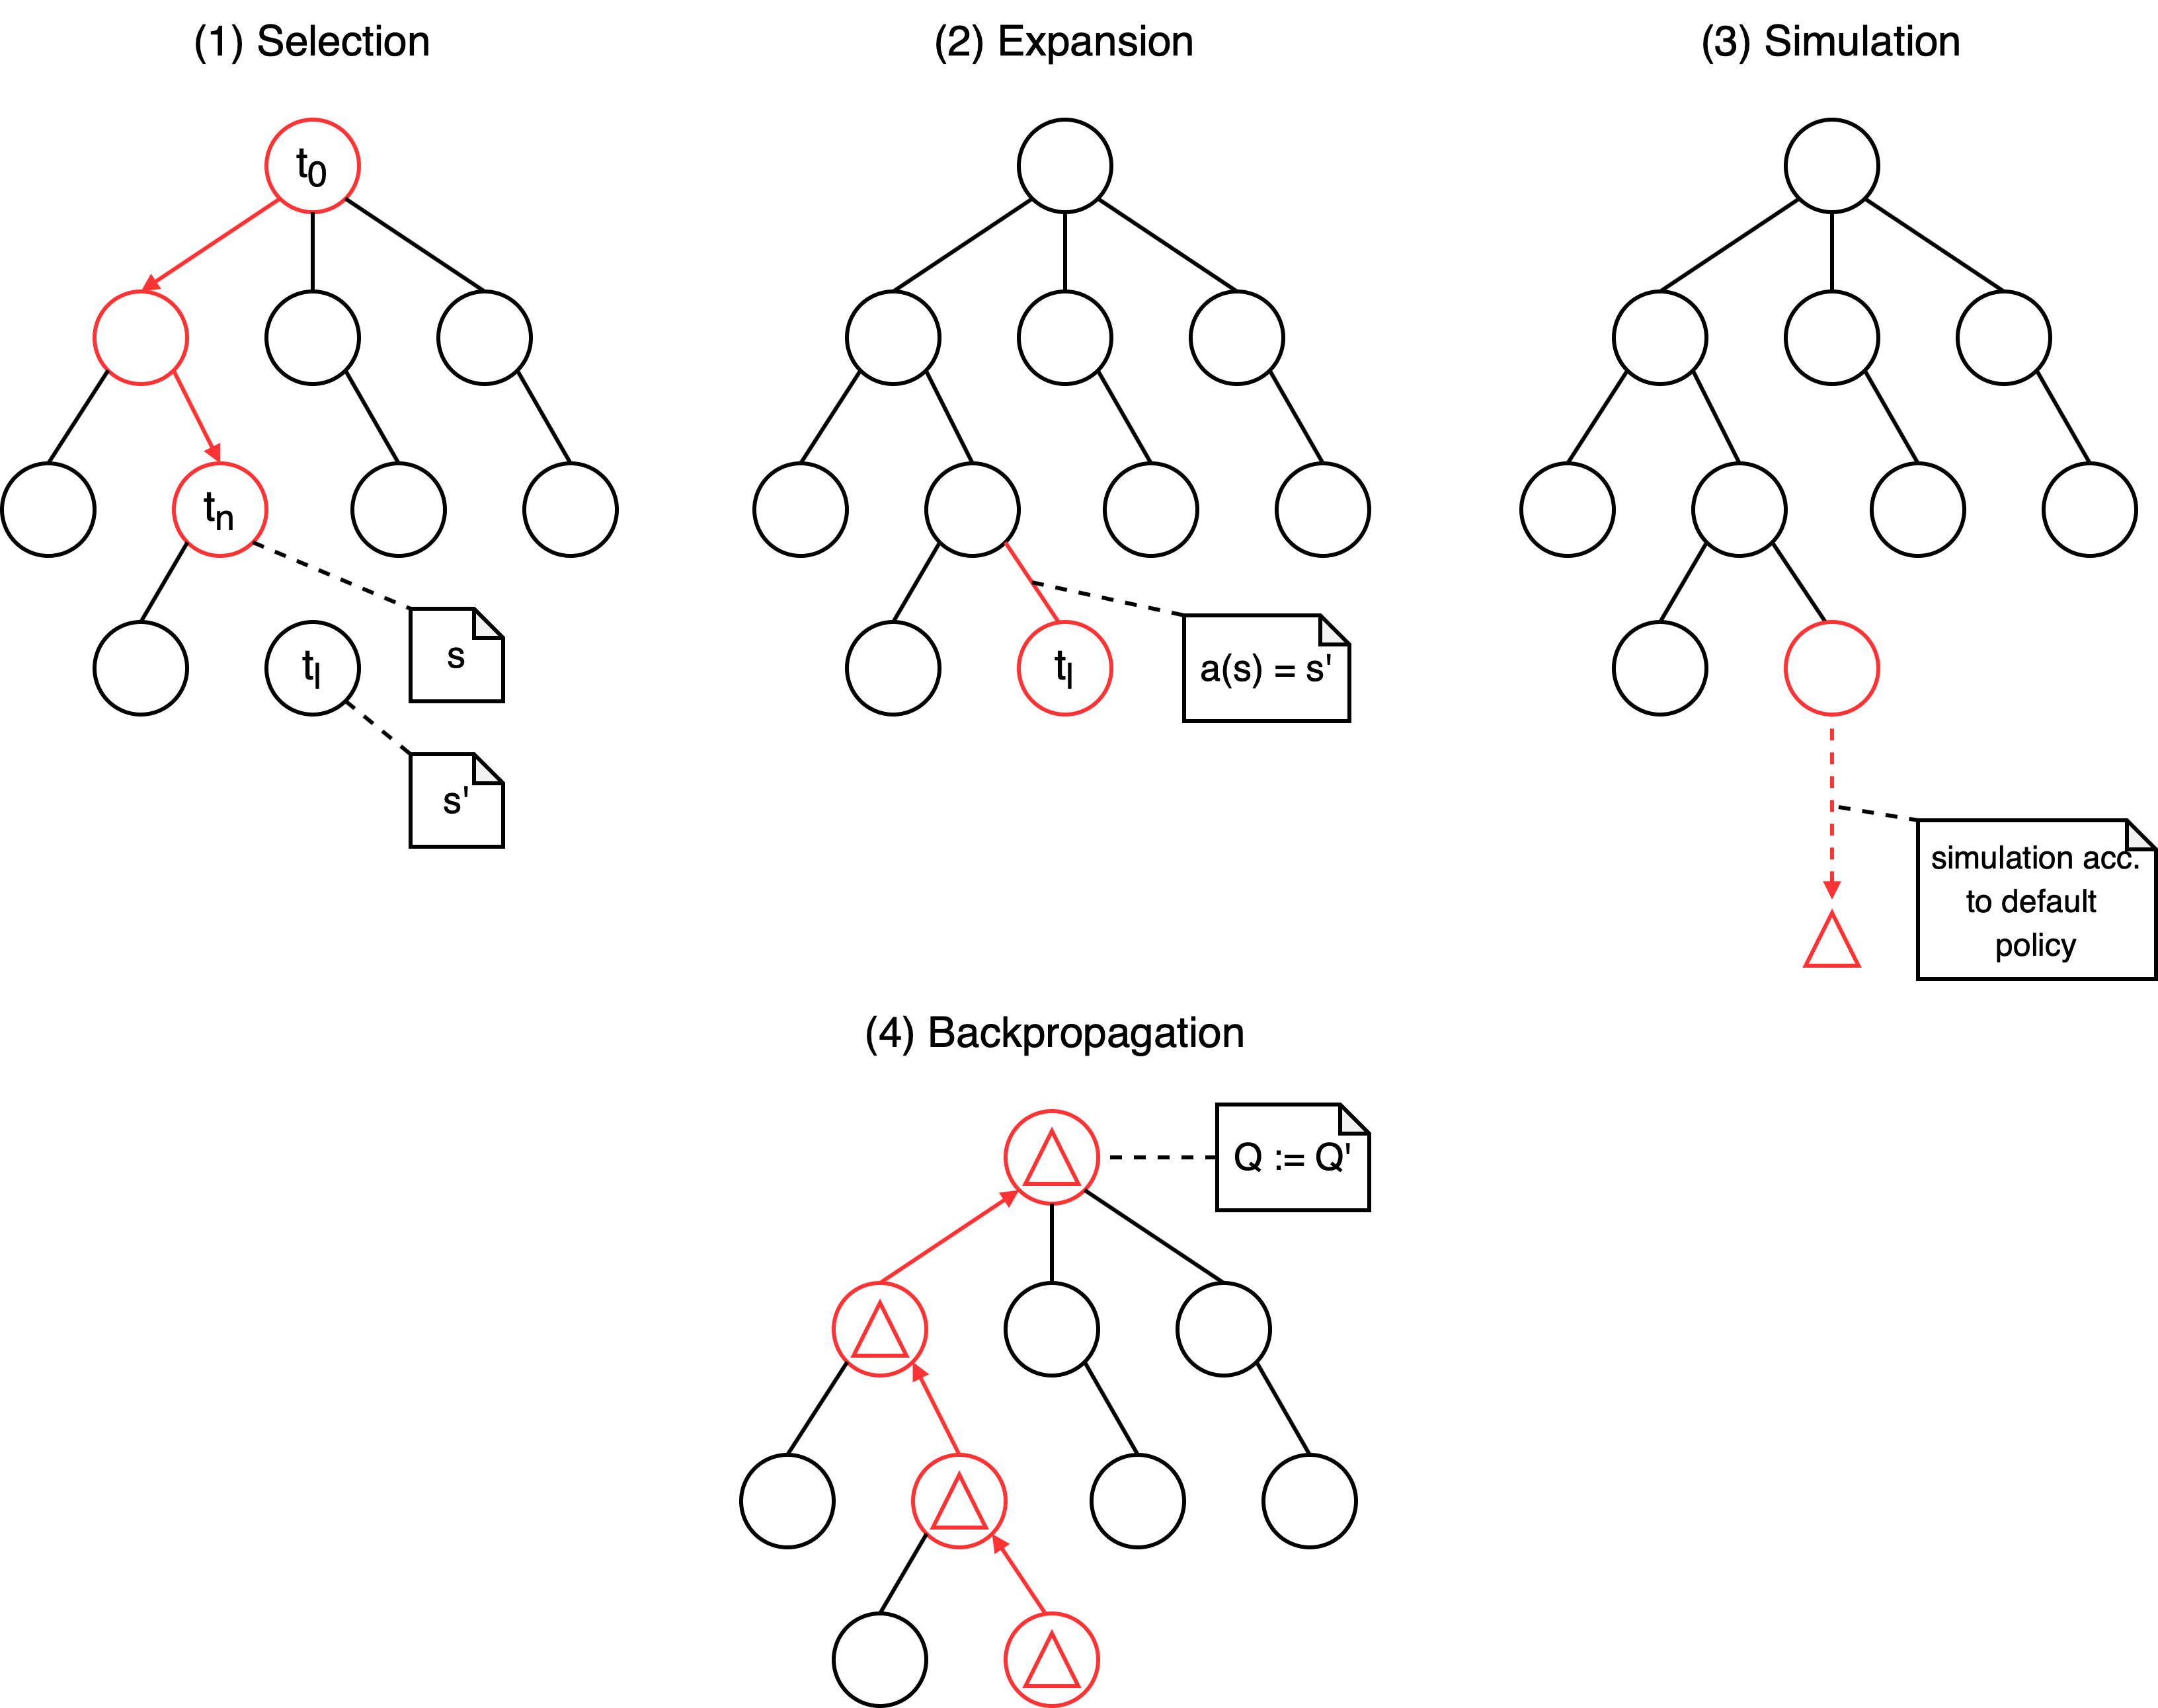
\includegraphics[width=0.8\textwidth]{img/mcts-basics.png}
    \caption{The four basic MCTS steps executed in each iteration. [modified image from \cite{browne2012survey}]}
    \label{fig:mcts_basics}
\end{figure}
How the game states are represented, if/how games need to be discretized and how the outcome of terminal states is evaluated is not part of the algorithm. 
\begin{algorithm}[ht!]
\begin{algorithmic}
\Function{MCTS}{$s_0$} 
    \State create root node $v_0$ with state $s_0$
    \While{within computational budget}
    \State $v_l \gets$ \Call{TreePolicy}{$v_0$} \Comment{$v_l$ is the last node reached}
    \State $\Delta \gets$ \Call{DefaultPolicy}{$s(v_l)$} \Comment{simulate from state node $v_l$ with state $s_l$}
    \State \Call{Backup}{$v_l,\Delta$}
    \EndWhile
    \State \Return \Call{$a$}{\Call{bestChild}{$v_0$}$)$} \Comment{return most valuable action $a$}
\EndFunction
\end{algorithmic}
\caption{Basic Monte Carlo Tree Search function.}
\label{alg:mcts_basic}
\end{algorithm}

Browne~et~al. \cite{browne2012survey} identify three characteristics of Monte Carlo Tree Search: \begin{enumerate*}[label=\alph*)]
    \item \textit{Aheuristic}: There is no concrete domain knowledge required. MCTS can be applied to any domain that can be modeled as a tree. However, any available knowledge can greatly improve the performance of the search, whether this manifests in modeling design decision of the problem itself or heuristics for use in the tree and/or simulation policy.   
    \item \textit{Anytime}: Due to the immediate backpropagation of each game outcome the values of all nodes are always up-to-date. This makes it possible to return (i.e., end the search and return the root action) at any time.
    \item \textit{Asymmetric}: Since more promising nodes are favored by the search the tree does not grow at the same rate (of iterations) everywhere. The tree can gain an irregular, asymmetric shape.
\end{enumerate*}
\subsection{Upper Confidence Bound For Trees}
\label{ss:uct}
Upper Confidence Bound for Trees (UCT) is an important family of MCTS-Algorithms that was first proposed by Kocsis and Szespevari \cite{kocsis2006bandit}. They follow the basic MCTS-schema shown in Algorithm \ref{alg:mcts_basic} but define their own default- and tree-policies. In the following we discuss an implementation of UCT in pseudocode for games (except for some changes in the nomenclature, UCT is of course applicable to all generic search problems). All possible states of the game are described using nodes, each node $v$ has four members:
\begin{itemize}
    \item associated state $s(v)$
    \item incoming action $a(v)$
    \item total simulation reward $Q(v)$
    \item visit count $N(v)$
\end{itemize} Initially all nodes except the initial state of the game are not part of the search tree but can be added (\enquote{chosen}) during the search. More precisely: While the budget is not exhausted a child node is selected according to the tree policy, which is discussed in detail below. Then the simulation is executed according to the default policy of choosing actions (and thus child nodes) uniformly at random. When a terminal state is reached the results are backpropagated and the four entries in the nodes are updated accordingly. When the budget is used up the best node is returned as a result. Relating to games, the result of the search is the best action possible from the root node (the \enquote{root action}).

A key concept of UCT is the treatment of child-node selection as a MAB-problem. With this abstraction we can use the UCB1 equation from above in the tree policy (see Algorithm \ref{alg:uct_tree_policy}):
\begin{equation*}
    UCT(v) = \frac{Q(v')}{N(v')}+C_p \cdot \sqrt{\frac{2 \ln N(v)}{N(v')}}
\end{equation*} The node $v'$ is a child of $v$. There are two differences to default UCB1. One is the treatment of $a$ and $s$ as nodes to fit the pseudocode. In the next sections we omit the treatment of $a(v)$ and $s(v)$ as members of a node for convenience and just write $a$ and $s$. Read \enquote{state $s$ represented by a node} and \enquote{action $a$ which leads to the state $s$ represented by a node}. More consequential however is the parameter $C_p > 0$ that mediates between exploration and exploitation. Usually we just set $C_p = \frac{1}{2} $ but this can of course be tuned. Now the child selection just translates to maximizing this function. UCT always chooses the child node $v^\star$ (or, more precisely, the action $a^\star$ leading to $v^\star$) with
\begin{equation*}
    v^\star = \underset{v' \in v.children}{\arg \max} UCT(v)
\end{equation*}  
\begin{algorithm}[ht!]
\begin{algorithmic}
\Function{TreePolicy}{$v$} 
    \While{$v$ is nonterminal}
    \If{v is not fully expanded}
    \State \Return{\Call{Expand}{$v$}}
    \Else
    \State $v \gets$ \Call{BestChild}{$v,C_p$}
    \EndIf
    \EndWhile
    \Return{$v$}
\EndFunction \\
\Function{Expand}{$v$}
\State choose untried $a \in A(s(v))$
\State add new child $v'$ to $v.children$ with $s(v') = f(s(v),a)$ and $a(v') = a$
\State \Return{$v'$}
\EndFunction \\
\Function{BestChild}{$v,c$}
\State \Return{$\underset{v' \in v.children}{\arg \max} \frac{Q(v')}{N(v')}+C_p \cdot \sqrt{\frac{2 \ln N(v)}{N(v')}}$}
\EndFunction
\end{algorithmic}
\caption{The tree policy of UCT.}
\label{alg:uct_tree_policy}
\end{algorithm}
\begin{algorithm}[ht!]
\begin{algorithmic}
\Function{DefaultPolicy}{$s$}
\While{$s$ is non-terminal}
\State choose $a \in A(s)$ uniformly at random
\State $s \gets f(s,a)$
\EndWhile
\State \Return{reward for $s$}
\EndFunction \\

\Function{Backup}{$v, \Delta$} \Comment{no strictly speaking part of the default policy}
\While{$v$ is not null}
\State $N(v) \gets N(v) + 1$
\State $Q(v) \gets Q(v) + \Delta(v,p)$
\State $v \gets v.parent$
\EndWhile
\State $N(v) \gets N(v) + 1$
\State $Q(v) \gets Q(v) + \Delta$
\State $\Delta \gets - \Delta$
\State $v \gets v.parent$
\EndFunction
\end{algorithmic}
\caption{The default policy of UCT.}
\label{alg:uct_default_policy}
\end{algorithm}
\subsection{Comparison to Other Algorithms}
The two most notable search search algorithms that can be viewed as direct alternatives to MCTS are \textit{Minimax}/\textit{Expectimax} and \textit{Alpha-Beta-Pruning}. While their relation to each other is clear (Alpha-Beta-Pruning is strictly better than Minimax since it is a generalization of the latter \cite{knuth1975analysis}) an apples-to-apples comparison of each to MCTS is difficult. Ramanujan et al. \cite{ramanujan2011behavior} show that there are both search spaces where MCTS significantly outperforms Minimax and ones where the exact opposite is true. They argue that this is due to the existence of trap states. That is, game states which are only a small number of moves away from defeat. In the real world this can be seen in the fact that while for playing Go (few traps) MCTS is a key success factor, in Chess (many traps) Minimax and its derivations are usually the better choice. On the other hand Kato et al. \cite{kato2015comparative} show that when it comes to other games like Amazons Alpha-Beta-Pruning yields better results. Additionally, Baier and Winands \cite{baier2014monte} argue that when comparing search algorithms the heuristics and evaluation functions used can massively influence the results and thus the choice depends on existing domain knowledge and not primarily on the basic algorithmic framework.
\FloatBarrier